\documentclass{standalone}
\usepackage{tikz}
\usepackage{ctex,siunitx}
\setCJKmainfont{Noto Serif CJK SC}
\usepackage{tkz-euclide}
\usepackage{amsmath}
\usetikzlibrary{patterns, calc,3d}
\usetikzlibrary {decorations.pathmorphing,decorations.pathreplacing,decorations.shapes}
\tikzset{label style/.append style={font=\small}}
\begin{document}
\small
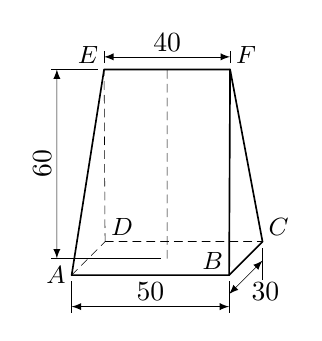
\begin{tikzpicture}[>=latex,scale=0.4,inner sep=2pt]
  \tkzDefPoints{0/0/A,5/0/B}
  \tkzDefShiftPoint[B](45:1.5){C}
  \tkzDefShiftPoint[A](45:1.5){D}
  \tkzDefMidPoint(A,C)\tkzGetPoint{H}
  \tkzDefShiftPoint[H](0,6){H'}
  \tkzDefShiftPoint[H](2,6){F}
  \tkzDefShiftPoint[H](-2,6){E}
  \tkzDrawPolygon[semithick](A,B,C,F,E)
  \tkzDrawSegments[semithick](B,F)
  \tkzDrawSegments[densely dashed](A,D D,E D,C H,H')
  \draw[very thin] ([yshift=2mm]E)--++(0,0.4)([yshift=2mm]F)--++(0,0.4);
  \draw[very thin,<->] ([yshift=4mm]E)--([yshift=4mm]F)node[midway,above]{40};
  \draw[very thin] ([xshift=-2mm]H)--++(-3.5,0)([xshift=-2mm]E)--++(-1.5,0);
  \draw[very thin,<->]([xshift=-35mm]H)--([xshift=-15mm]E)node[midway,sloped,above,rotate=180]{60};
  \draw[very thin] ([yshift=-2mm]A)--++(0,-1)([yshift=-2mm]B)--++(0,-1)([yshift=-2mm]C)--++(0,-1);
  \draw[very thin,<->] ([yshift=-10mm]A)--([yshift=-10mm]B)node[midway,above]{50};
  \draw[very thin,<->] ([yshift=-6mm]B)--([yshift=-6mm]C)node[midway,below right]{30};
  \tkzLabelPoints[above left](E,B)
  \tkzLabelPoints[above right](F,C,D)
  \tkzLabelPoints[left](A)
\end{tikzpicture}
\end{document}